\section{Introducción}

\textbf{La productividad laboral no solo varía entre actividades económicas, sino también entre territorios.} El Informe 01 de esta serie mostró que el crecimiento de la productividad en Colombia fue muy distinto entre ramas de actividad económica. Este informe toma esa misma preocupación y la lleva al plano territorial: ¿en qué departamentos creció más la producción por trabajador y por hora trabajada?

\textbf{La productividad refleja condiciones que no son iguales en todo el país.} La geografía, la infraestructura, la formación de los trabajadores, la informalidad, la conectividad y la capacidad institucional cambian de manera importante entre departamentos. Por eso, dos territorios pueden tener trayectorias muy distintas de productividad.

\textbf{El objetivo de este informe es medir la evolución de la productividad laboral departamental en Colombia entre 2010 y 2024pr.} Para ello se combina el PIB departamental del DANE, expresado en pesos constantes de 2015, con ocupados y horas trabajadas de la Gran Encuesta Integrada de Hogares (GEIH). El ejercicio se concentra en los 24 departamentos que pueden seguirse de manera comparable durante todo el periodo.

\textbf{El informe está organizado en seis secciones, incluyendo esta introducción.} La sección 2 presenta la metodología y las fuentes. La sección 3 compara la productividad laboral de los departamentos. La sección 4 distingue entre niveles y crecimientos de la productividad usando una gráfica de cuadrantes y un ejercicio descriptivo de convergencia. La sección 5 analiza la relación entre crecimiento del trabajo y crecimiento de la productividad. La sección 6 presenta conclusiones. El apéndice incluye el detalle de cada departamento.

\section{Metodología}

\textbf{La medición combina cuentas nacionales departamentales y microdatos de la GEIH.} El numerador corresponde al PIB departamental real del DANE, tomado del anexo \textit{Producto Interno Bruto por departamento}, en series encadenadas de volumen con año de referencia 2015. El denominador se construye con la GEIH. El número de ocupados corresponde al promedio anual de personas ocupadas, calculado con el factor de expansión de la encuesta.

\textbf{Las horas trabajadas se calculan a partir del promedio observado de horas semanales.} Para cada departamento y año se calcula el promedio ponderado de horas semanales entre los ocupados que reportan horas válidas. Ese promedio se multiplica por el número total de ocupados del departamento y se anualiza por 52 semanas. De esta manera, los ocupados que no reportan horas no se tratan implícitamente como trabajadores con cero horas, sino que se les asigna el promedio observado del respectivo departamento y año.

\textbf{El informe se concentra en 24 departamentos comparables durante todo el periodo.} La GEIH permite seguir de manera consistente los departamentos tradicionales del diseño muestral entre 2010 y 2025. Para evitar imputaciones o cambios artificiales en la cobertura, se excluyen San Andrés y Providencia y los departamentos de la Amazonía y la Orinoquía que no hacen parte de ese panel comparable desde 2010. Bogotá D.C. se trata como departamento porque así aparece en las cuentas nacionales departamentales.

\textbf{Se construyen dos indicadores de productividad laboral.} El PIB por trabajador divide el PIB real departamental entre el número anual de ocupados del departamento. El PIB por hora trabajada divide el mismo PIB entre el total anual de horas trabajadas. Esta segunda medida permite distinguir si un aumento del producto por trabajador proviene de producir más por hora o de trabajar más horas.

\textbf{El periodo de análisis es 2010--2024pr y se excluye 2020.} El año 2020 se excluye para mantener consistencia con el tratamiento del Informe 01, dado que la base anual de GEIH usada en el proyecto no considera ese año como comparable. Las tasas de crecimiento reportadas son tasas anualizadas entre 2010 y 2024pr.

\section{Productividad laboral por departamento}

\textbf{La productividad laboral departamental presenta diferencias importantes en niveles y en crecimientos.} Conviene comenzar por los niveles, porque muestran la jerarquía territorial de productividad en 2024pr. El Cuadro \ref{tab:pib_geih_productividad_departamento_ranking_niveles} ordena los departamentos según su PIB por trabajador y su PIB por hora trabajada.

\begin{table}[H]
\centering
\caption{Ranking departamental de niveles de productividad laboral, 2024pr}
\label{tab:pib_geih_productividad_departamento_ranking_niveles}
\scriptsize
\begin{tabular}{lrrrr}
\toprule
Departamento & PIB/trab. 2024pr & Puesto & PIB/hora 2024pr & Puesto \\
\midrule
Bogotá D.C. & 67,4 & 1 & 28,6 & 1 \\
Santander & 62,0 & 3 & 26,1 & 2 \\
Meta & 63,1 & 2 & 25,9 & 3 \\
Valle del Cauca & 54,5 & 4 & 23,4 & 4 \\
Boyacá & 47,5 & 6 & 22,6 & 5 \\
Antioquia & 47,7 & 5 & 20,3 & 6 \\
Bolívar & 45,1 & 7 & 19,8 & 7 \\
Cundinamarca & 40,4 & 8 & 17,4 & 8 \\
Tolima & 40,0 & 9 & 16,9 & 9 \\
Risaralda & 38,7 & 10 & 16,4 & 10 \\
Atlántico & 37,3 & 11 & 16,0 & 11 \\
Caldas & 36,6 & 12 & 15,6 & 12 \\
Quindío & 33,8 & 13 & 15,1 & 13 \\
Huila & 31,6 & 15 & 14,2 & 14 \\
Cesar & 32,6 & 14 & 13,8 & 15 \\
Cauca & 26,6 & 17 & 13,7 & 16 \\
Chocó & 28,6 & 16 & 11,9 & 17 \\
La Guajira & 24,8 & 19 & 11,1 & 18 \\
Córdoba & 22,0 & 22 & 10,7 & 19 \\
Caquetá & 24,9 & 18 & 10,5 & 20 \\
Sucre & 22,0 & 23 & 10,4 & 21 \\
Magdalena & 23,9 & 21 & 10,3 & 22 \\
Norte de Santander & 24,3 & 20 & 10,0 & 23 \\
Nariño & 17,8 & 24 & 9,1 & 24 \\
\bottomrule
\end{tabular}
\caption*{\footnotesize Nota: PIB por trabajador en millones de pesos constantes de 2015; PIB por hora en miles de pesos constantes de 2015. La tabla está ordenada por el nivel de PIB por hora trabajada en 2024pr. Fuente: cálculos propios con DANE y GEIH.}
\end{table}

\textbf{El ranking de niveles muestra una jerarquía territorial bastante clara.} Bogotá D.C. ocupa el primer lugar tanto en PIB por trabajador como en PIB por hora trabajada. Santander, Meta y Valle del Cauca también se ubican entre los departamentos con mayor productividad en 2024pr. En el extremo inferior aparecen Nariño, Norte de Santander, Magdalena, Sucre y Caquetá cuando se mide el PIB por hora. Este ordenamiento es importante porque varios de los departamentos que más crecieron durante el periodo todavía parten de niveles bajos de productividad.

\textbf{Los niveles de productividad en 2024pr muestran brechas territoriales relevantes.} Bogotá D.C. registró un PIB por hora de 28,6 miles de pesos de 2015, Santander de 26,1 y Meta de 25,9. En contraste, Nariño, Norte de Santander, Magdalena, Sucre y Caquetá se ubicaron cerca o por debajo de 10,5 miles de pesos de 2015 por hora trabajada. Esto confirma que los departamentos con mayor crecimiento no necesariamente son los departamentos con mayores niveles de productividad.

\textbf{Después de mirar los niveles, el Cuadro \ref{tab:pib_geih_productividad_departamento} muestra cómo cambió la productividad departamental.} La tabla ordena los departamentos por crecimiento del PIB por hora trabajada entre 2010 y 2024pr. La lectura conjunta del PIB por trabajador y el PIB por hora es útil porque algunos departamentos pueden mostrar mejoras por trabajador aun cuando parte de esa mejora provenga de cambios en las horas trabajadas.

\begin{table}[H]
\centering
\caption{Productividad laboral por departamento, 2010--2024pr}
\label{tab:pib_geih_productividad_departamento}
\scriptsize
\begin{tabular}{lrrrr}
\toprule
Departamento & PIB/trab. 2024pr & PIB/hora 2024pr & Crec. PIB/trab. & Crec. PIB/hora \\
\midrule
Quindío & 33,8 & 15,1 & 3,78\% & 4,63\% \\
Caquetá & 24,9 & 10,5 & 3,71\% & 4,17\% \\
Risaralda & 38,7 & 16,4 & 3,14\% & 3,51\% \\
Chocó & 28,6 & 11,9 & 2,95\% & 3,20\% \\
Caldas & 36,6 & 15,6 & 2,14\% & 2,57\% \\
Valle del Cauca & 54,5 & 23,4 & 2,15\% & 2,50\% \\
Sucre & 22,0 & 10,4 & 1,67\% & 2,45\% \\
Bogotá D.C. & 67,4 & 28,6 & 1,98\% & 2,44\% \\
Bolívar & 45,1 & 19,8 & 1,69\% & 2,34\% \\
Tolima & 40,0 & 16,9 & 2,04\% & 2,17\% \\
Cauca & 26,6 & 13,7 & 1,44\% & 2,05\% \\
Santander & 62,0 & 26,1 & 1,71\% & 1,96\% \\
Nariño & 17,8 & 9,1 & 0,97\% & 1,92\% \\
Córdoba & 22,0 & 10,7 & 0,90\% & 1,71\% \\
Antioquia & 47,7 & 20,3 & 1,27\% & 1,58\% \\
Boyacá & 47,5 & 22,6 & 1,16\% & 1,43\% \\
Norte de Santander & 24,3 & 10,0 & 1,23\% & 1,41\% \\
Magdalena & 23,9 & 10,3 & 0,16\% & 0,88\% \\
Atlántico & 37,3 & 16,0 & 0,46\% & 0,85\% \\
Cesar & 32,6 & 13,8 & -0,03\% & 0,57\% \\
Meta & 63,1 & 25,9 & 0,05\% & 0,55\% \\
Huila & 31,6 & 14,2 & -0,13\% & 0,11\% \\
Cundinamarca & 40,4 & 17,4 & -0,32\% & -0,14\% \\
La Guajira & 24,8 & 11,1 & -0,80\% & -0,51\% \\
\bottomrule
\end{tabular}
\caption*{\footnotesize Nota: PIB por trabajador en millones de pesos constantes de 2015; PIB por hora en miles de pesos constantes de 2015. Bogotá se trata como departamento. El universo corresponde a los 24 departamentos con información comparable en la GEIH para todo el periodo. Se excluye 2020 por no contar con GEIH anual comparable en la base del proyecto. Fuente: cálculos propios con DANE, Cuentas Nacionales Departamentales, y GEIH.}
\end{table}

\textbf{Los departamentos con mayor crecimiento del PIB por hora trabajada fueron Quindío, Caquetá y Risaralda.} En Quindío, el PIB por hora creció 4,63\% anual y el PIB por trabajador 3,78\% anual. En Caquetá, el PIB por hora creció 4,17\% anual y el PIB por trabajador 3,71\% anual. Risaralda también presentó un crecimiento alto en ambas medidas. Estos resultados muestran que algunos departamentos con niveles de productividad todavía bajos lograron avances importantes durante el periodo.

\textbf{En el otro extremo se ubican Cundinamarca y La Guajira.} Cundinamarca registra una caída anual de 0,14\% en el PIB por hora y de 0,32\% en el PIB por trabajador. La Guajira presenta una caída de 0,51\% en el PIB por hora y de 0,80\% en el PIB por trabajador. En estos casos, el crecimiento del trabajo no estuvo acompañado por un aumento proporcional del PIB real departamental.

\begin{figure}[H]
  \centering
  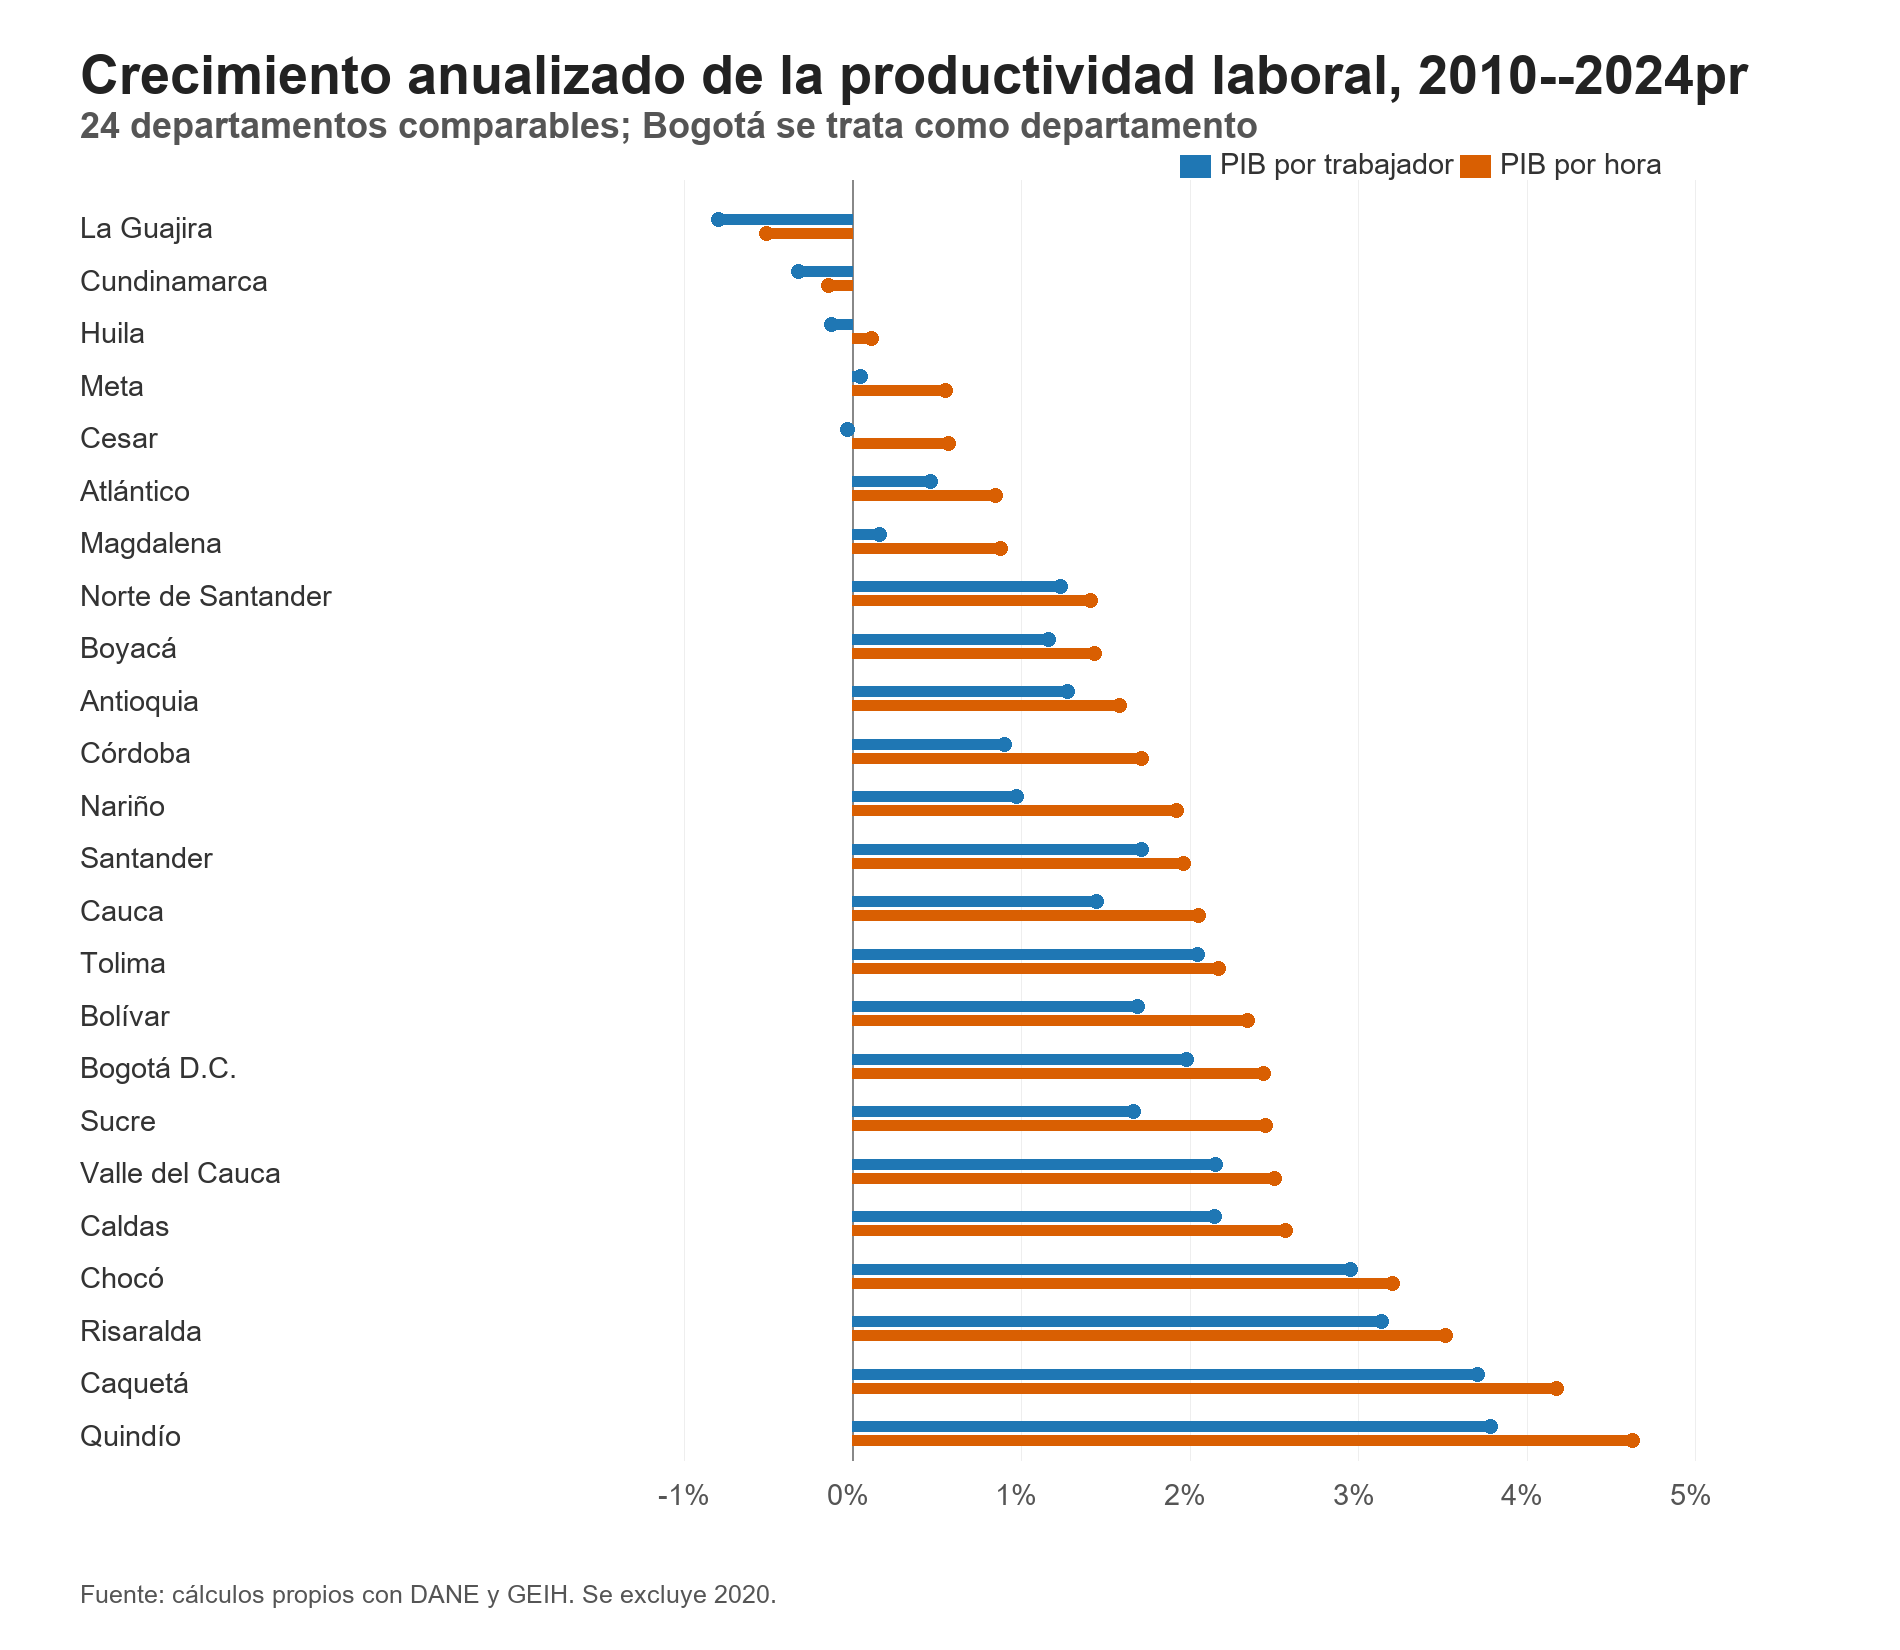
\includegraphics[width=\textwidth]{Paper/figures/fig_pib_geih_productividad_departamento.png}
  \caption{Crecimiento anualizado de la productividad laboral por departamento, 2010--2024pr}
  \label{fig:pib_geih_productividad_departamento}
\end{figure}

\textbf{La Figura \ref{fig:pib_geih_productividad_departamento} permite ver que las diferencias no son marginales.} La distancia entre los departamentos de mayor y menor crecimiento supera cinco puntos porcentuales anuales cuando se mide la productividad por hora. El desempeño agregado del país, por tanto, oculta trayectorias territoriales muy distintas.

\section{Niveles, crecimientos y convergencia}

\textbf{La comparación entre niveles y crecimientos ayuda a ordenar mejor el diagnóstico territorial.} La Figura \ref{fig:pib_geih_productividad_departamento_cuadrantes} cruza el crecimiento anualizado del PIB por hora trabajada entre 2010 y 2024pr con el nivel de PIB por hora en 2024pr. La línea vertical marca el crecimiento del agregado de los 24 departamentos y la línea horizontal marca su nivel de productividad por hora en 2024pr.

\begin{figure}[H]
  \centering
  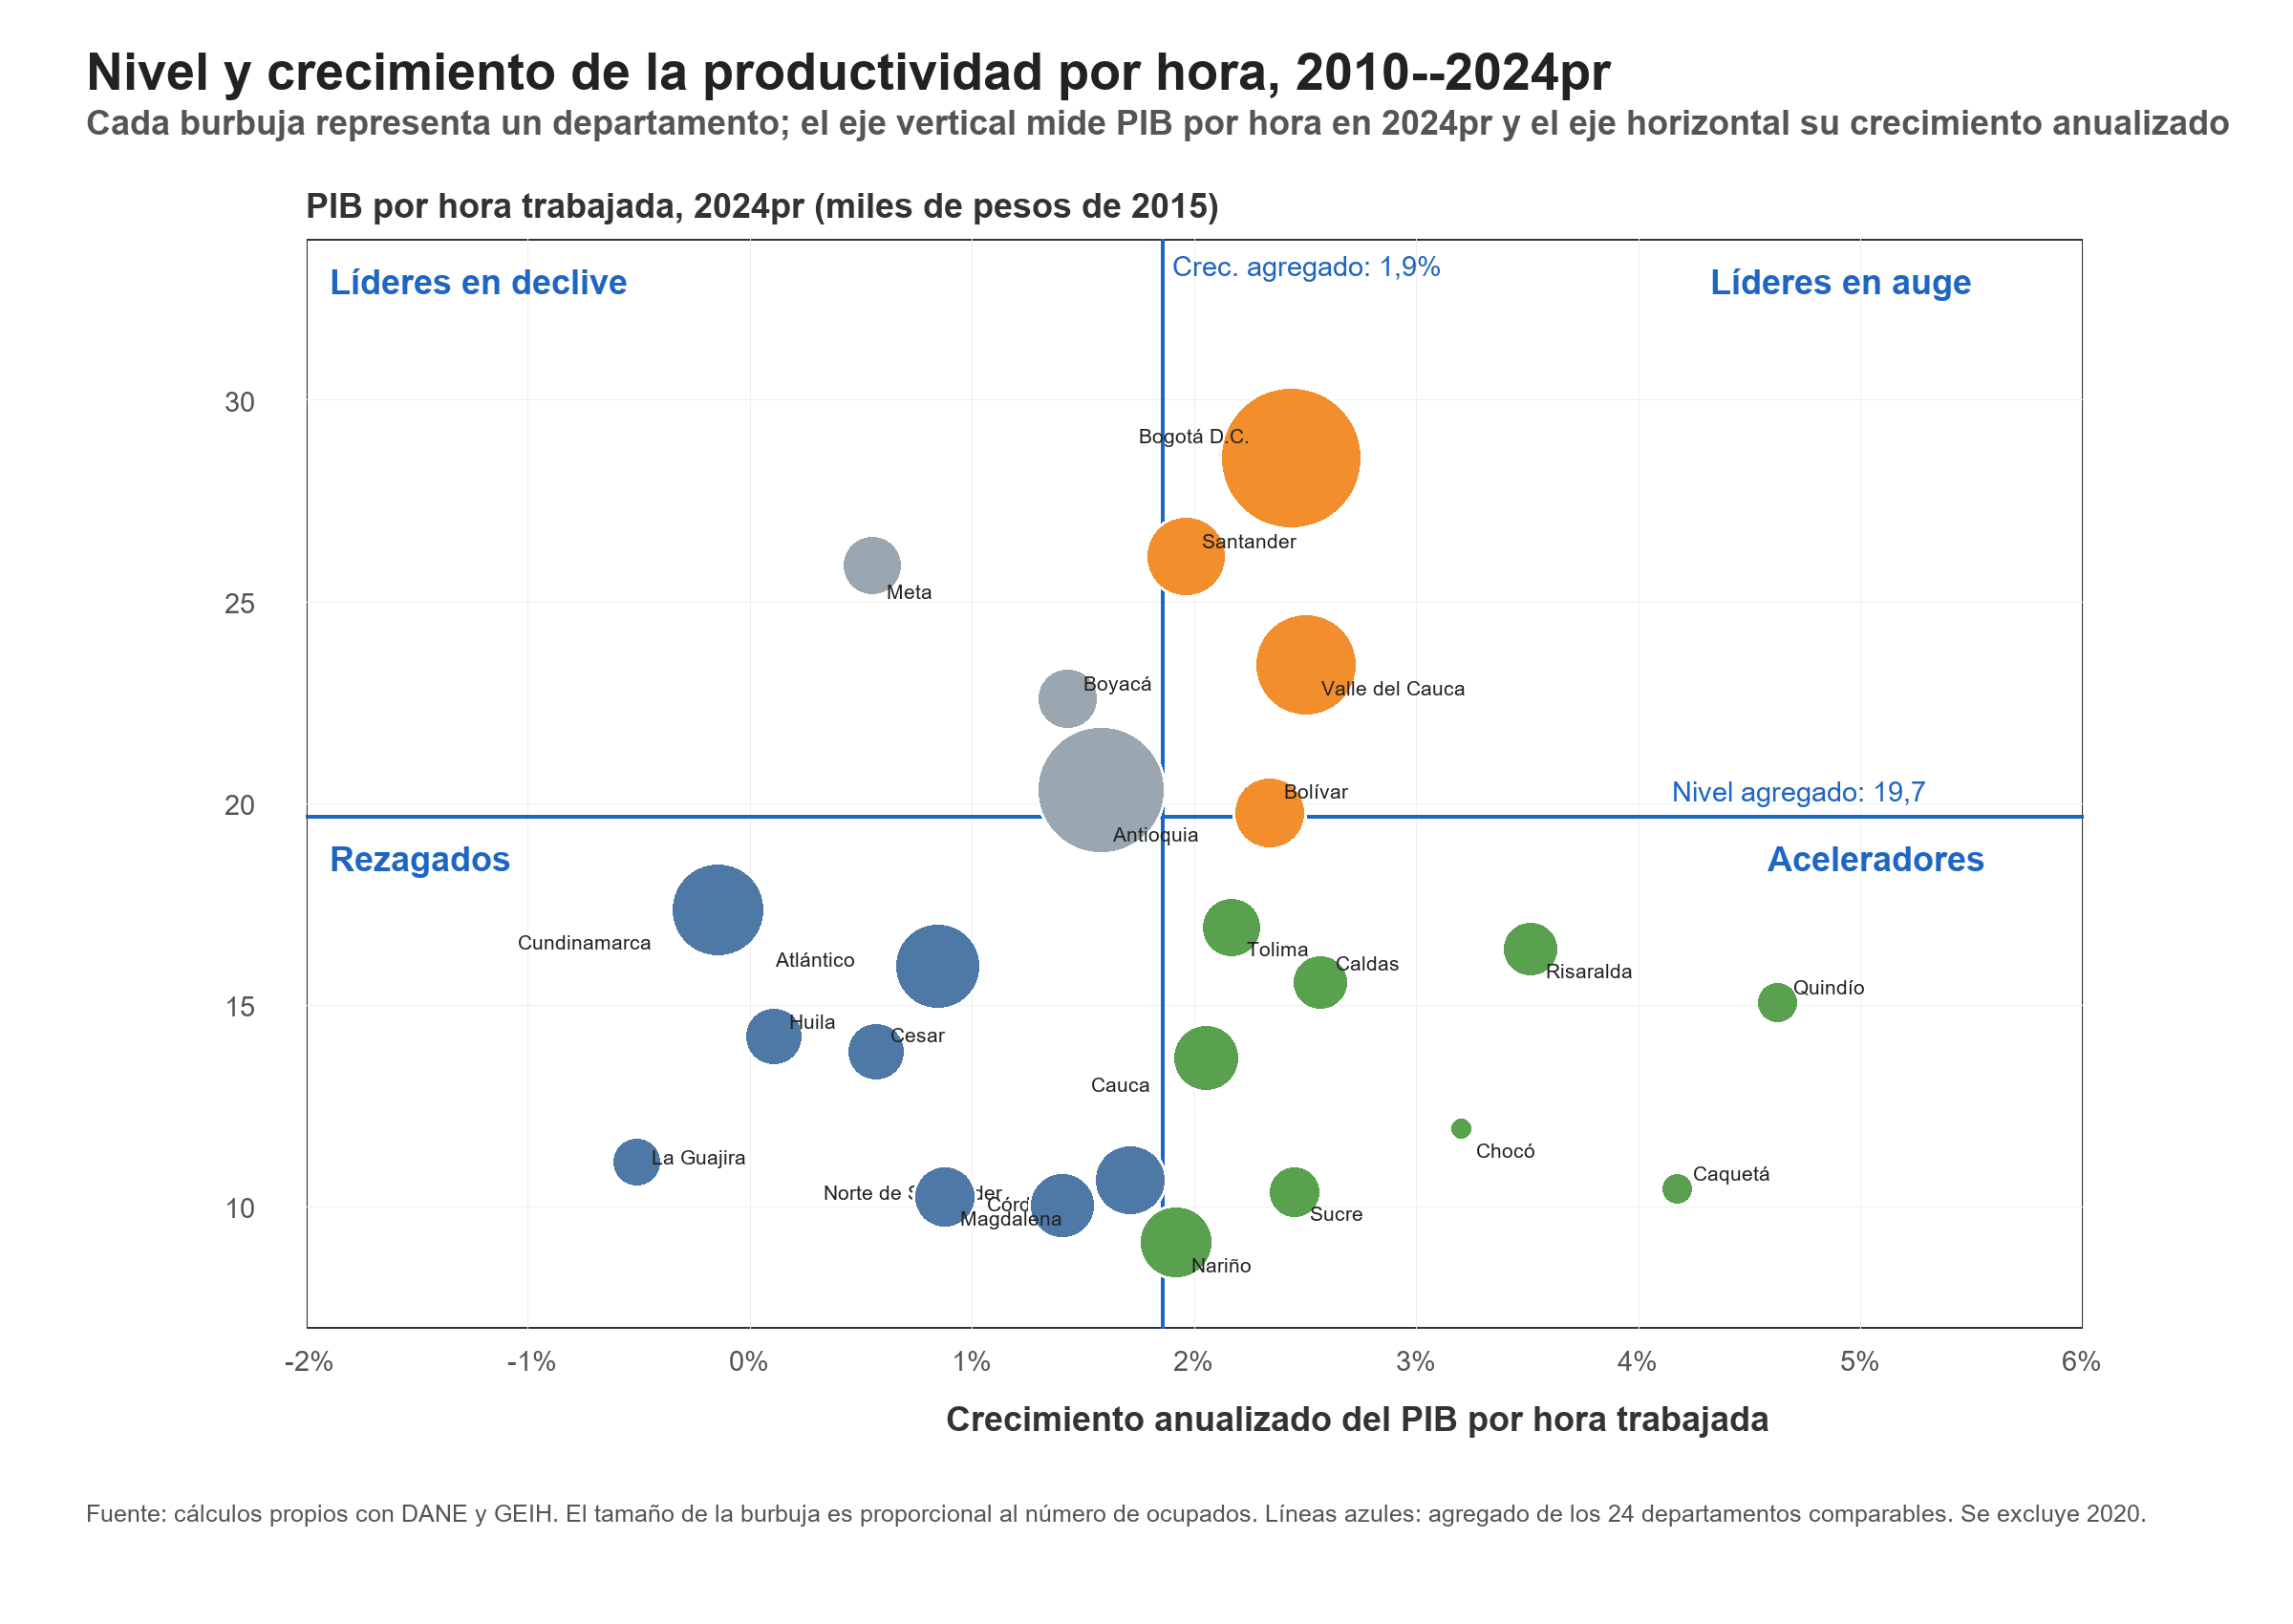
\includegraphics[width=\textwidth]{Paper/figures/fig_pib_geih_productividad_departamento_cuadrantes.png}
  \caption{Nivel y crecimiento de la productividad por hora por departamento, 2010--2024pr}
  \label{fig:pib_geih_productividad_departamento_cuadrantes}
  \caption*{\footnotesize Nota: la línea vertical muestra el crecimiento agregado del PIB por hora trabajada y la línea horizontal muestra el nivel agregado de PIB por hora en 2024pr. El tamaño de la burbuja es proporcional al número de ocupados del departamento. Fuente: cálculos propios con DANE y GEIH.}
\end{figure}

\textbf{Los cuadrantes muestran cuatro situaciones distintas.} Bogotá D.C., Santander, Valle del Cauca y Bolívar aparecen como líderes en auge: tienen un nivel de PIB por hora superior al agregado y, además, crecieron por encima del agregado. Meta, Boyacá y Antioquia aparecen como líderes en declive relativo: mantienen niveles altos de productividad, pero su crecimiento fue inferior al del agregado. Quindío, Caquetá, Risaralda, Chocó, Caldas y Sucre aparecen como aceleradores: tienen niveles bajos o medios de productividad, pero crecieron con fuerza. Finalmente, Cundinamarca, Atlántico, Huila, Cesar, Magdalena y La Guajira se ubican entre los rezagados: tienen niveles de productividad por hora inferiores al agregado y también crecieron por debajo de él.

\textbf{Esta clasificación no debe interpretarse como un ranking definitivo de desempeño departamental.} Un departamento puede crecer rápido porque parte de un nivel bajo, porque cambia su composición productiva, porque pierde empleos de baja productividad o porque recibe choques positivos en actividades específicas. Aun así, la figura es útil porque obliga a separar dos preguntas distintas: qué departamentos son más productivos y en cuáles está creciendo más la productividad.

\textbf{El ejercicio de convergencia muestra una relación negativa entre el nivel inicial de productividad y su crecimiento posterior.} La Figura \ref{fig:pib_geih_productividad_departamento_convergencia} compara el nivel de productividad de cada departamento en 2010 con su crecimiento anualizado entre 2010 y 2024pr. La correlación es negativa tanto para el PIB por trabajador (-0,33) como para el PIB por hora (-0,42). Esto sugiere que, en promedio, los departamentos que partieron de niveles más bajos tendieron a crecer más rápido.

\begin{figure}[H]
  \centering
  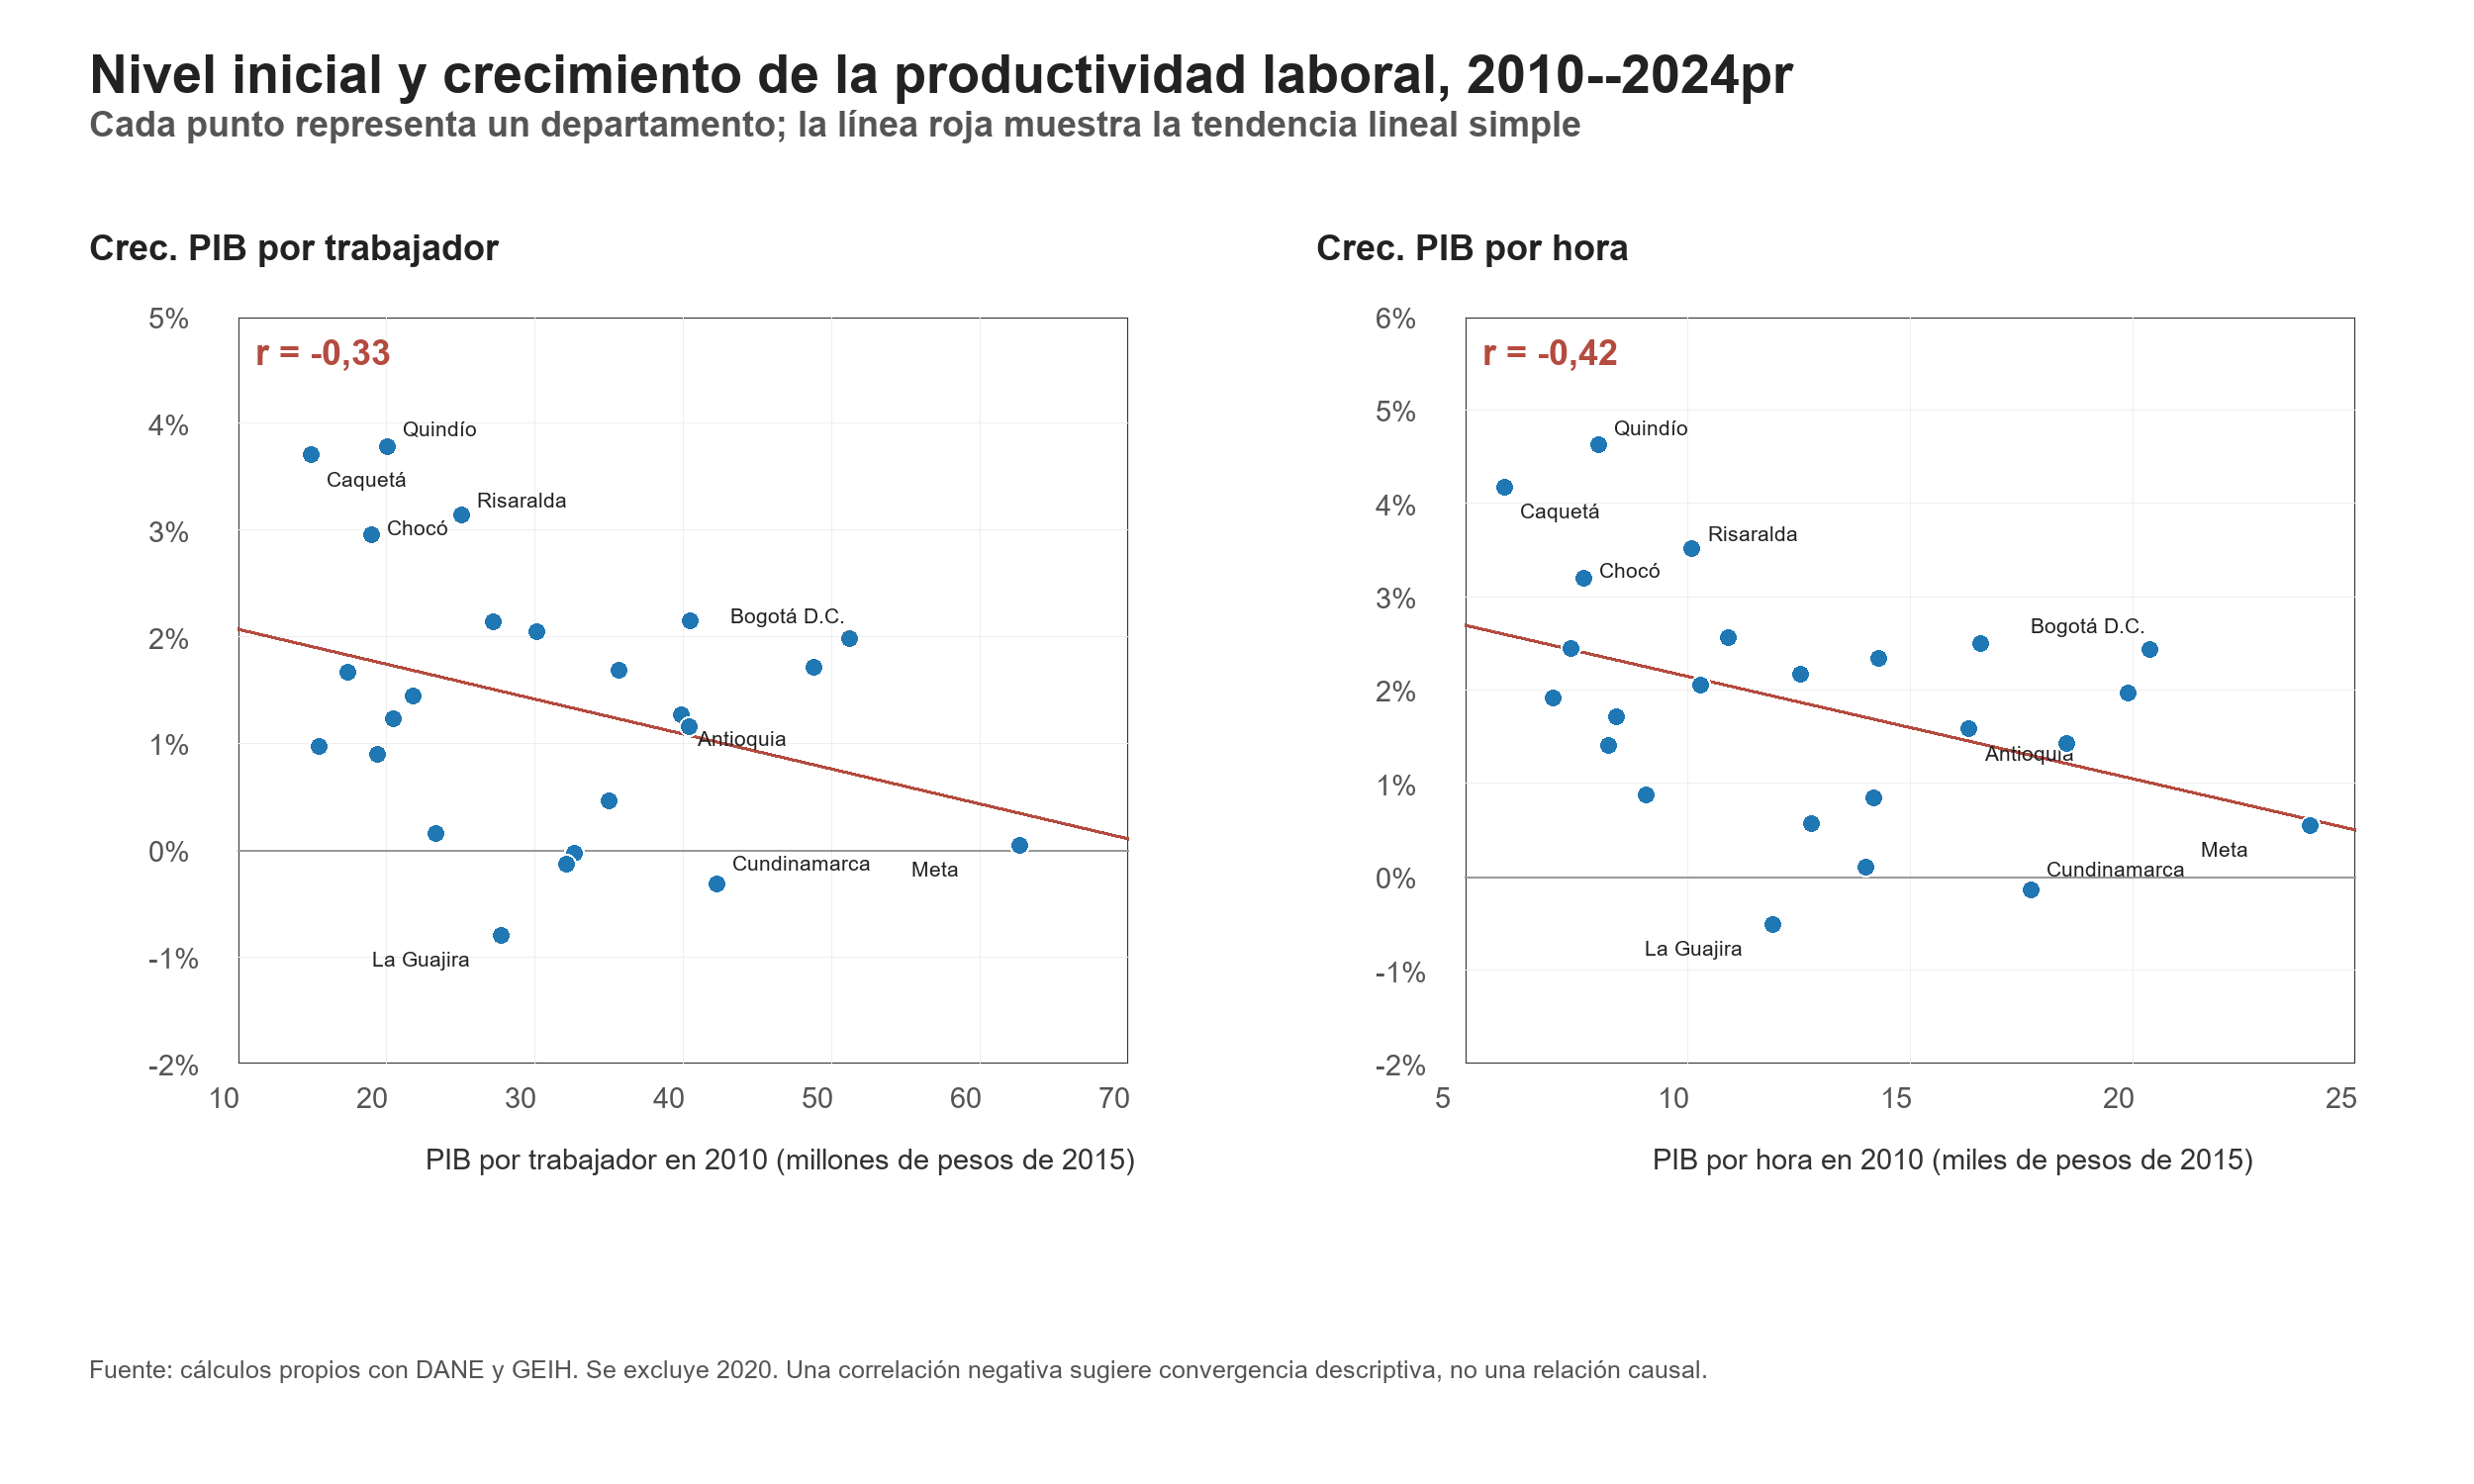
\includegraphics[width=\textwidth]{Paper/figures/fig_pib_geih_productividad_departamento_convergencia.png}
  \caption{Nivel inicial y crecimiento de la productividad laboral departamental, 2010--2024pr}
  \label{fig:pib_geih_productividad_departamento_convergencia}
\end{figure}

\textbf{La velocidad estimada de convergencia sugiere que el cierre de brechas territoriales sería lento.} Para aproximar esta velocidad se estima una relación descriptiva entre el crecimiento anualizado de la productividad y el logaritmo de su nivel inicial en 2010. El ejercicio no debe interpretarse como una estimación causal ni estructural, sino como una forma resumida de cuantificar el patrón observado en la Figura \ref{fig:pib_geih_productividad_departamento_convergencia}.

\begin{table}[H]
\centering
\caption{Velocidad descriptiva de convergencia departamental, 2010--2024pr}
\label{tab:pib_geih_productividad_departamento_velocidad_convergencia}
\small
\begin{tabular}{lrrr}
\toprule
Indicador & Corr. nivel inicial-crec. & Velocidad anual & Vida media \\
\midrule
PIB por trabajador & -0,36 & 1,22\% & 56,8 años \\
PIB por hora trabajada & -0,47 & 1,72\% & 40,4 años \\
\bottomrule
\end{tabular}
\caption*{\footnotesize Nota: la velocidad se calcula a partir de una regresión descriptiva entre el crecimiento logarítmico anualizado de la productividad y el logaritmo del nivel inicial de productividad en 2010, usando los 24 departamentos comparables. La vida media indica el número aproximado de años que tomaría cerrar la mitad de la brecha inicial si la velocidad estimada se mantuviera constante. Fuente: cálculos propios con DANE y GEIH.}
\end{table}

\textbf{La convergencia observada es parcial y debe interpretarse con cuidado.} Quindío, Caquetá, Risaralda y Chocó partieron de niveles relativamente bajos y registraron crecimientos altos de productividad. En sentido contrario, Meta partió de un nivel alto y tuvo un crecimiento bajo. Sin embargo, la relación no es mecánica: Bogotá D.C. partió de un nivel alto y aun así creció por encima del agregado, mientras que La Guajira partió de un nivel bajo y registró una caída en la productividad. Por eso, la figura debe leerse como evidencia descriptiva de convergencia parcial, no como una prueba de que las brechas territoriales estén cerrándose de manera generalizada. Incluso si se toma literalmente, la velocidad estimada implica que cerrar la mitad de la brecha inicial tomaría alrededor de 40 años para el PIB por hora y casi 57 años para el PIB por trabajador.

\section{Crecimiento del trabajo y crecimiento de la productividad}

\textbf{Una pregunta natural es si la ocupación creció más en los departamentos donde también creció más la productividad.} Esta relación importa porque el crecimiento económico se fortalece cuando el trabajo se expande en territorios donde la producción por trabajador o por hora también aumenta. En cambio, si el empleo crece en territorios con productividad estancada o decreciente, el aumento del producto puede depender más de absorber trabajo que de producir más eficientemente.

\begin{table}[H]
\centering
\caption{Correlaciones departamentales seleccionadas sobre crecimiento y productividad}
\label{tab:pib_geih_productividad_departamento_correlaciones}
\begin{tabular}{llr}
\toprule
Variable 1 & Variable 2 & Correlación \\
\midrule
Crec. ocupados & Crec. PIB por trabajador & -0,78 \\
Crec. ocupados & Crec. PIB por hora & -0,73 \\
Crec. horas totales & Crec. PIB por trabajador & -0,80 \\
Crec. horas totales & Crec. PIB por hora & -0,78 \\
PIB por trabajador inicial & Crec. PIB por trabajador & -0,33 \\
PIB por hora inicial & Crec. PIB por hora & -0,42 \\
\bottomrule
\end{tabular}
\caption*{\footnotesize Nota: correlaciones de Pearson calculadas entre los 24 departamentos comparables, tratando a Bogotá como departamento. Fuente: cálculos propios con DANE y GEIH.}
\end{table}

\begin{figure}[H]
  \centering
  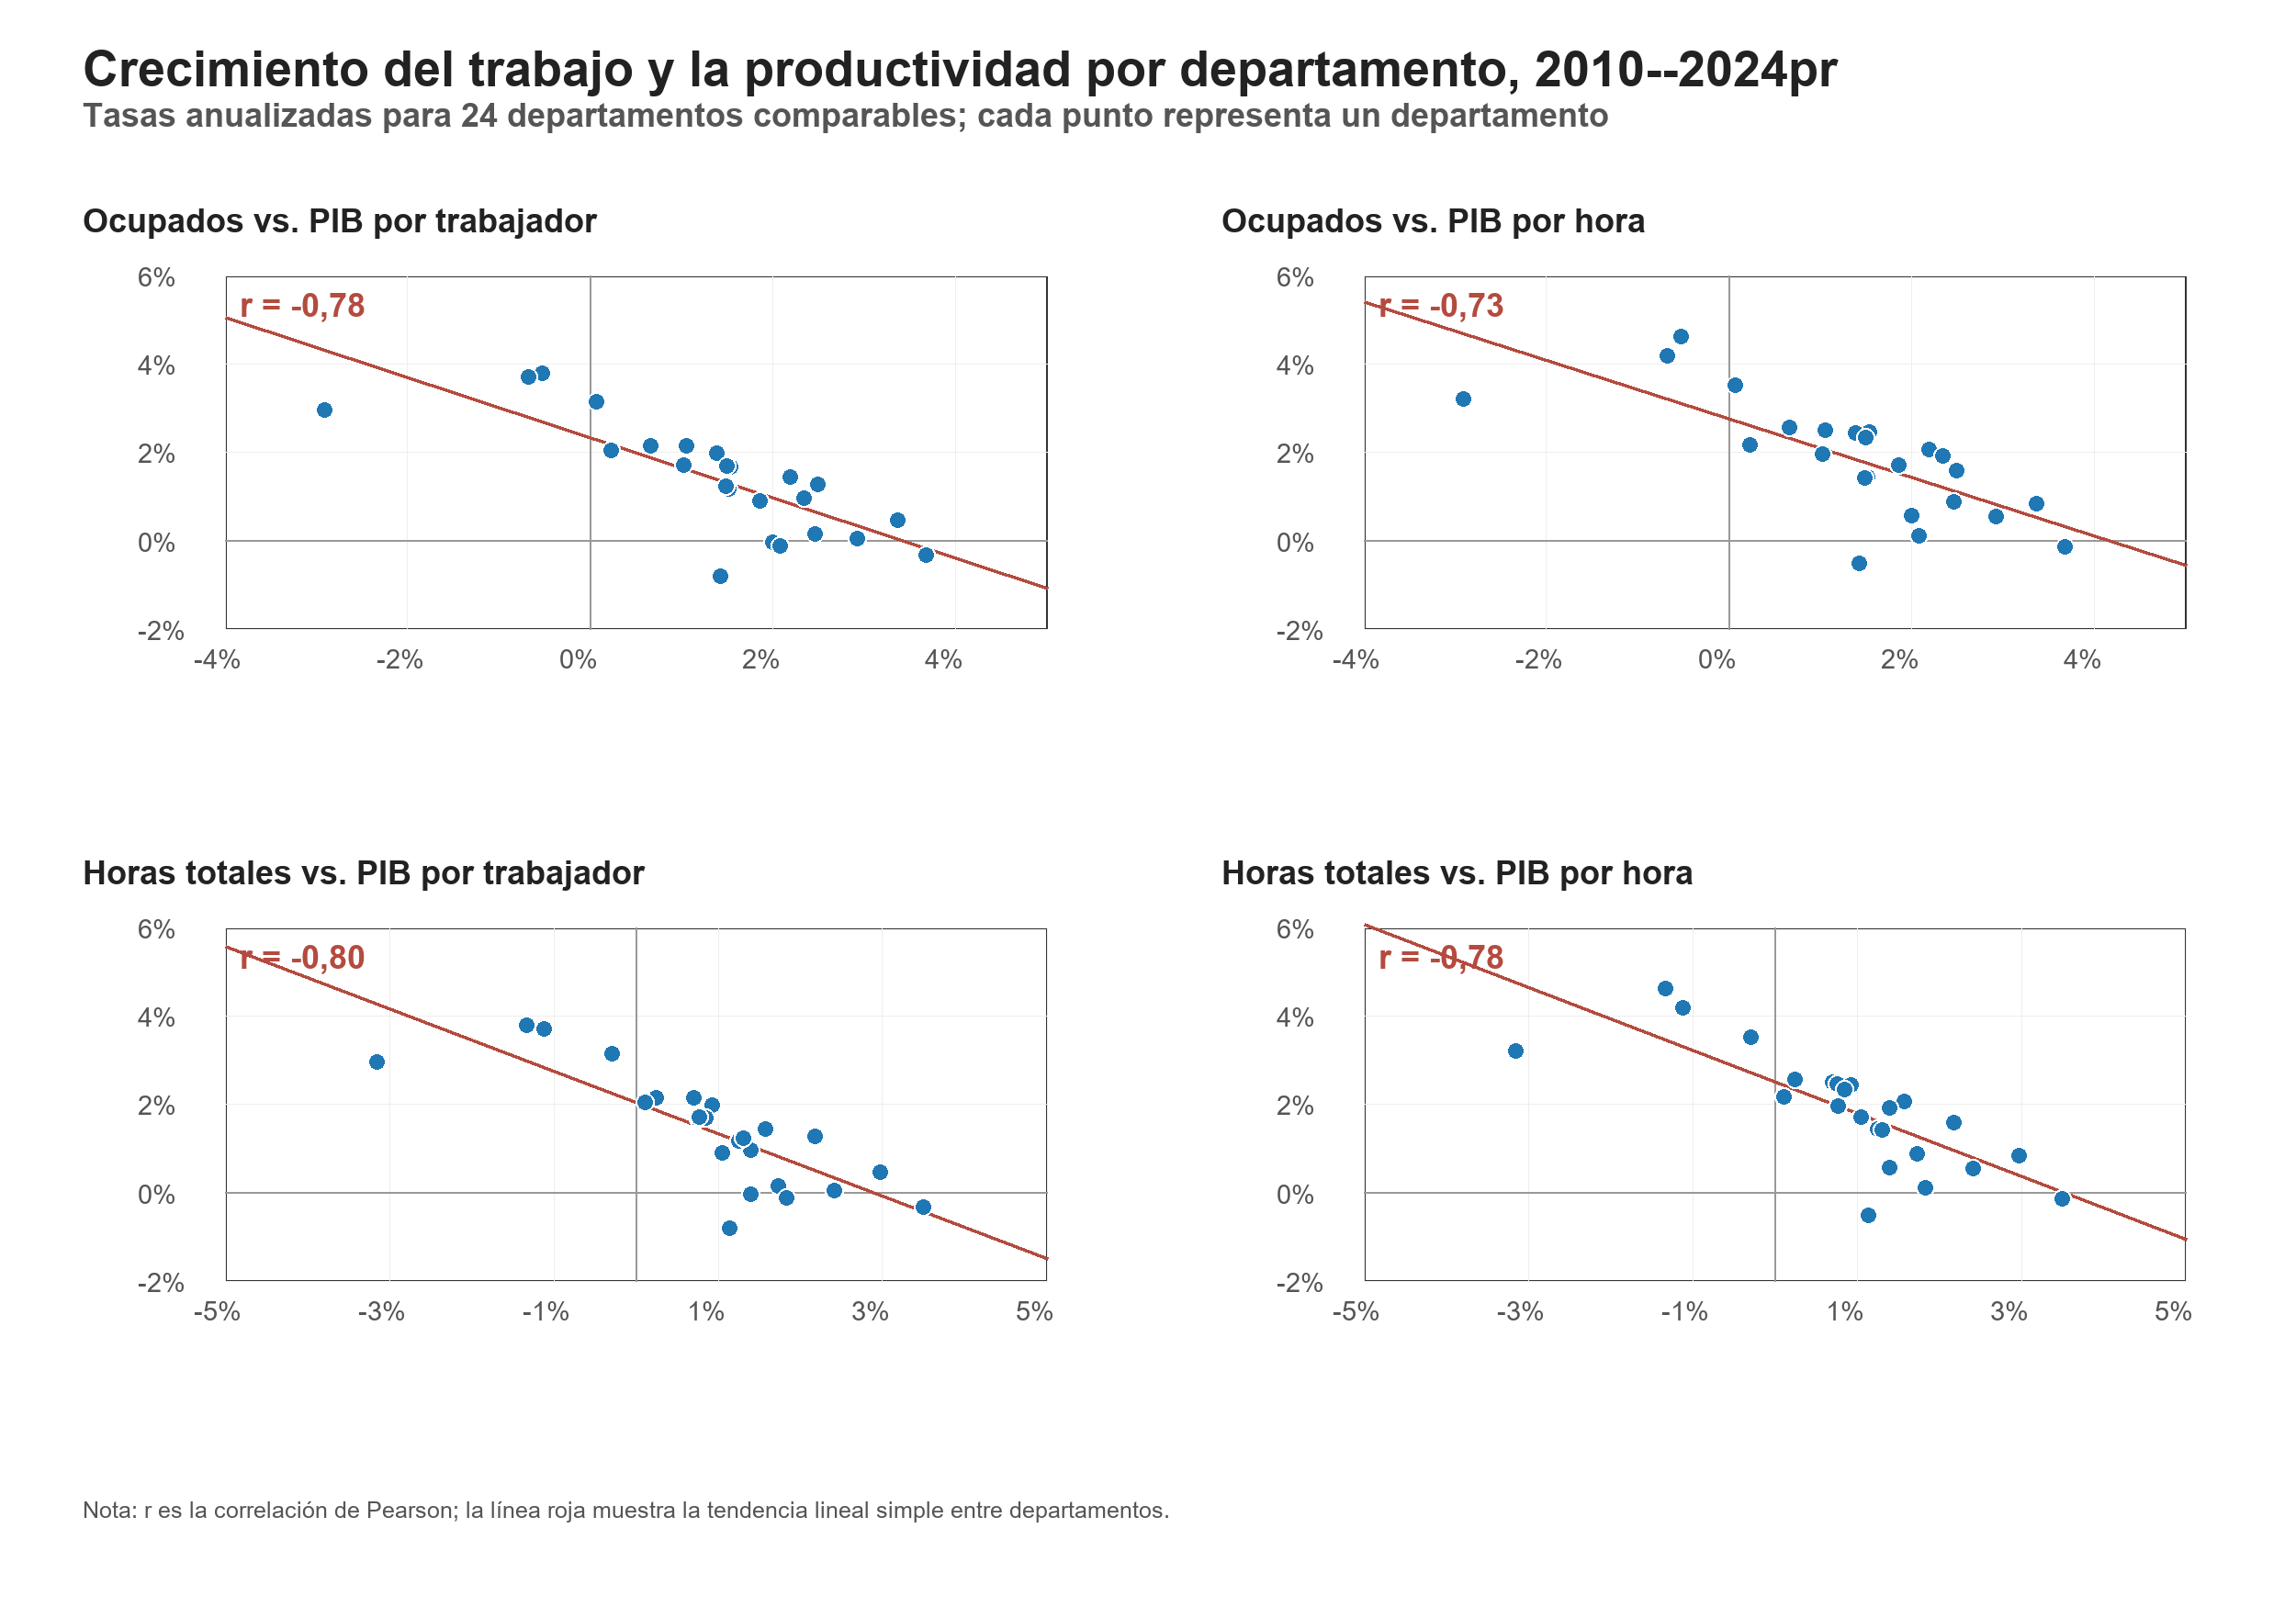
\includegraphics[width=\textwidth]{Paper/figures/fig_pib_geih_productividad_departamento_correlaciones.png}
  \caption{Crecimiento del trabajo y crecimiento de la productividad por departamento}
  \label{fig:pib_geih_productividad_departamento_correlaciones}
\end{figure}

\textbf{Los resultados sugieren que el crecimiento del trabajo y el crecimiento de la productividad no avanzaron de la mano.} La correlación entre el crecimiento de los ocupados y el crecimiento del PIB por hora fue negativa. Departamentos como Cundinamarca, Atlántico y Meta aumentaron sus ocupados a ritmos relativamente altos, pero registraron un crecimiento débil o negativo del PIB por hora. En contraste, Quindío, Caquetá y Chocó tuvieron alto crecimiento de productividad con caídas o bajo crecimiento de ocupados.

\textbf{Esta relación debe interpretarse con cautela.} No prueba por sí sola que el trabajo se haya asignado mal entre departamentos. Puede reflejar migración, cambios en la composición sectorial, variaciones en la intensidad horaria o choques específicos en actividades dominantes de cada territorio. Sin embargo, sí plantea una pregunta importante para la política pública: qué condiciones permiten que el crecimiento del empleo ocurra junto con aumentos sostenidos de producción por hora.

\section{Conclusiones}

\textbf{El análisis departamental muestra que la productividad laboral colombiana tiene una dimensión territorial fuerte.} Incluso al limitar el ejercicio a los 24 departamentos comparables, las diferencias en niveles y crecimientos son amplias. Esto implica que la agenda de productividad no puede limitarse a una lectura nacional promedio.

\textbf{Hay señales de convergencia territorial, pero estas son parciales, desiguales y lentas.} Los departamentos que partieron con menores niveles de productividad tendieron, en promedio, a crecer más rápido. Este patrón se observa en Quindío, Caquetá, Risaralda y Chocó. Sin embargo, la relación no es mecánica: Bogotá D.C. partió de un nivel alto y siguió creciendo por encima del agregado, mientras que La Guajira partió de un nivel bajo y registró una caída en productividad. La velocidad descriptiva de convergencia es cercana a 1,7\% anual para el PIB por hora y a 1,2\% anual para el PIB por trabajador. Por eso, el ejercicio sugiere convergencia descriptiva, pero no permite concluir que las brechas territoriales se estén cerrando de manera rápida o generalizada.

\textbf{La productividad por hora ofrece una lectura más precisa que la productividad por trabajador cuando las horas trabajadas cambian.} En varios departamentos, el crecimiento del PIB por trabajador y el crecimiento del PIB por hora no son idénticos porque las horas semanales por trabajador se movieron durante el periodo. La distinción es relevante para evaluar si la mejora de productividad implica producir más eficientemente o simplemente trabajar más horas.

\textbf{El crecimiento de ocupados no siempre se concentró en los departamentos con mayor crecimiento de productividad.} Esta evidencia no prueba por sí sola una mala asignación territorial del trabajo, pero sí señala una pregunta importante para la política pública: qué condiciones permiten que el empleo y la productividad crezcan al mismo tiempo. La agenda territorial no puede limitarse a generar más empleo; también debe preguntarse qué tipo de empleo se está creando, en qué actividades y bajo qué condiciones de capital, infraestructura y capacidades productivas.

\textbf{Una agenda territorial de productividad debe identificar los mecanismos detrás de estas diferencias.} Entre los candidatos están la composición sectorial, la infraestructura, la calidad del empleo, la informalidad, la educación, la inversión privada y la capacidad de los territorios para conectar empresas y trabajadores con mercados más amplios. Este informe ofrece una primera medición descriptiva para orientar ese diagnóstico.
